% Options for packages loaded elsewhere
\PassOptionsToPackage{unicode}{hyperref}
\PassOptionsToPackage{hyphens}{url}
\PassOptionsToPackage{dvipsnames,svgnames,x11names}{xcolor}
%
\documentclass[
  letterpaper,
]{article}

\usepackage{amsmath,amssymb}
\usepackage{lmodern}
\usepackage{iftex}
\ifPDFTeX
  \usepackage[T1]{fontenc}
  \usepackage[utf8]{inputenc}
  \usepackage{textcomp} % provide euro and other symbols
\else % if luatex or xetex
  \usepackage{unicode-math}
  \defaultfontfeatures{Scale=MatchLowercase}
  \defaultfontfeatures[\rmfamily]{Ligatures=TeX,Scale=1}
\fi
% Use upquote if available, for straight quotes in verbatim environments
\IfFileExists{upquote.sty}{\usepackage{upquote}}{}
\IfFileExists{microtype.sty}{% use microtype if available
  \usepackage[]{microtype}
  \UseMicrotypeSet[protrusion]{basicmath} % disable protrusion for tt fonts
}{}
\makeatletter
\@ifundefined{KOMAClassName}{% if non-KOMA class
  \IfFileExists{parskip.sty}{%
    \usepackage{parskip}
  }{% else
    \setlength{\parindent}{0pt}
    \setlength{\parskip}{6pt plus 2pt minus 1pt}}
}{% if KOMA class
  \KOMAoptions{parskip=half}}
\makeatother
\usepackage{xcolor}
\setlength{\emergencystretch}{3em} % prevent overfull lines
\setcounter{secnumdepth}{3}
% Make \paragraph and \subparagraph free-standing
\ifx\paragraph\undefined\else
  \let\oldparagraph\paragraph
  \renewcommand{\paragraph}[1]{\oldparagraph{#1}\mbox{}}
\fi
\ifx\subparagraph\undefined\else
  \let\oldsubparagraph\subparagraph
  \renewcommand{\subparagraph}[1]{\oldsubparagraph{#1}\mbox{}}
\fi

\usepackage{color}
\usepackage{fancyvrb}
\newcommand{\VerbBar}{|}
\newcommand{\VERB}{\Verb[commandchars=\\\{\}]}
\DefineVerbatimEnvironment{Highlighting}{Verbatim}{commandchars=\\\{\}}
% Add ',fontsize=\small' for more characters per line
\newenvironment{Shaded}{}{}
\newcommand{\AlertTok}[1]{\textcolor[rgb]{1.00,0.33,0.33}{\textbf{#1}}}
\newcommand{\AnnotationTok}[1]{\textcolor[rgb]{0.42,0.45,0.49}{#1}}
\newcommand{\AttributeTok}[1]{\textcolor[rgb]{0.84,0.23,0.29}{#1}}
\newcommand{\BaseNTok}[1]{\textcolor[rgb]{0.00,0.36,0.77}{#1}}
\newcommand{\BuiltInTok}[1]{\textcolor[rgb]{0.84,0.23,0.29}{#1}}
\newcommand{\CharTok}[1]{\textcolor[rgb]{0.01,0.18,0.38}{#1}}
\newcommand{\CommentTok}[1]{\textcolor[rgb]{0.42,0.45,0.49}{#1}}
\newcommand{\CommentVarTok}[1]{\textcolor[rgb]{0.42,0.45,0.49}{#1}}
\newcommand{\ConstantTok}[1]{\textcolor[rgb]{0.00,0.36,0.77}{#1}}
\newcommand{\ControlFlowTok}[1]{\textcolor[rgb]{0.84,0.23,0.29}{#1}}
\newcommand{\DataTypeTok}[1]{\textcolor[rgb]{0.84,0.23,0.29}{#1}}
\newcommand{\DecValTok}[1]{\textcolor[rgb]{0.00,0.36,0.77}{#1}}
\newcommand{\DocumentationTok}[1]{\textcolor[rgb]{0.42,0.45,0.49}{#1}}
\newcommand{\ErrorTok}[1]{\textcolor[rgb]{1.00,0.33,0.33}{\underline{#1}}}
\newcommand{\ExtensionTok}[1]{\textcolor[rgb]{0.84,0.23,0.29}{\textbf{#1}}}
\newcommand{\FloatTok}[1]{\textcolor[rgb]{0.00,0.36,0.77}{#1}}
\newcommand{\FunctionTok}[1]{\textcolor[rgb]{0.44,0.26,0.76}{#1}}
\newcommand{\ImportTok}[1]{\textcolor[rgb]{0.01,0.18,0.38}{#1}}
\newcommand{\InformationTok}[1]{\textcolor[rgb]{0.42,0.45,0.49}{#1}}
\newcommand{\KeywordTok}[1]{\textcolor[rgb]{0.84,0.23,0.29}{#1}}
\newcommand{\NormalTok}[1]{\textcolor[rgb]{0.14,0.16,0.18}{#1}}
\newcommand{\OperatorTok}[1]{\textcolor[rgb]{0.14,0.16,0.18}{#1}}
\newcommand{\OtherTok}[1]{\textcolor[rgb]{0.44,0.26,0.76}{#1}}
\newcommand{\PreprocessorTok}[1]{\textcolor[rgb]{0.84,0.23,0.29}{#1}}
\newcommand{\RegionMarkerTok}[1]{\textcolor[rgb]{0.42,0.45,0.49}{#1}}
\newcommand{\SpecialCharTok}[1]{\textcolor[rgb]{0.00,0.36,0.77}{#1}}
\newcommand{\SpecialStringTok}[1]{\textcolor[rgb]{0.01,0.18,0.38}{#1}}
\newcommand{\StringTok}[1]{\textcolor[rgb]{0.01,0.18,0.38}{#1}}
\newcommand{\VariableTok}[1]{\textcolor[rgb]{0.89,0.38,0.04}{#1}}
\newcommand{\VerbatimStringTok}[1]{\textcolor[rgb]{0.01,0.18,0.38}{#1}}
\newcommand{\WarningTok}[1]{\textcolor[rgb]{1.00,0.33,0.33}{#1}}

\providecommand{\tightlist}{%
  \setlength{\itemsep}{0pt}\setlength{\parskip}{0pt}}\usepackage{longtable,booktabs,array}
\usepackage{calc} % for calculating minipage widths
% Correct order of tables after \paragraph or \subparagraph
\usepackage{etoolbox}
\makeatletter
\patchcmd\longtable{\par}{\if@noskipsec\mbox{}\fi\par}{}{}
\makeatother
% Allow footnotes in longtable head/foot
\IfFileExists{footnotehyper.sty}{\usepackage{footnotehyper}}{\usepackage{footnote}}
\makesavenoteenv{longtable}
\usepackage{graphicx}
\makeatletter
\def\maxwidth{\ifdim\Gin@nat@width>\linewidth\linewidth\else\Gin@nat@width\fi}
\def\maxheight{\ifdim\Gin@nat@height>\textheight\textheight\else\Gin@nat@height\fi}
\makeatother
% Scale images if necessary, so that they will not overflow the page
% margins by default, and it is still possible to overwrite the defaults
% using explicit options in \includegraphics[width, height, ...]{}
\setkeys{Gin}{width=\maxwidth,height=\maxheight,keepaspectratio}
% Set default figure placement to htbp
\makeatletter
\def\fps@figure{htbp}
\makeatother

\makeatletter
\makeatother
\makeatletter
\makeatother
\makeatletter
\@ifpackageloaded{caption}{}{\usepackage{caption}}
\AtBeginDocument{%
\ifdefined\contentsname
  \renewcommand*\contentsname{Table of contents}
\else
  \newcommand\contentsname{Table of contents}
\fi
\ifdefined\listfigurename
  \renewcommand*\listfigurename{List of Figures}
\else
  \newcommand\listfigurename{List of Figures}
\fi
\ifdefined\listtablename
  \renewcommand*\listtablename{List of Tables}
\else
  \newcommand\listtablename{List of Tables}
\fi
\ifdefined\figurename
  \renewcommand*\figurename{Figure}
\else
  \newcommand\figurename{Figure}
\fi
\ifdefined\tablename
  \renewcommand*\tablename{Table}
\else
  \newcommand\tablename{Table}
\fi
}
\@ifpackageloaded{float}{}{\usepackage{float}}
\floatstyle{ruled}
\@ifundefined{c@chapter}{\newfloat{codelisting}{h}{lop}}{\newfloat{codelisting}{h}{lop}[chapter]}
\floatname{codelisting}{Listing}
\newcommand*\listoflistings{\listof{codelisting}{List of Listings}}
\makeatother
\makeatletter
\@ifpackageloaded{caption}{}{\usepackage{caption}}
\@ifpackageloaded{subcaption}{}{\usepackage{subcaption}}
\makeatother
\makeatletter
\@ifpackageloaded{tcolorbox}{}{\usepackage[many]{tcolorbox}}
\makeatother
\makeatletter
\@ifundefined{shadecolor}{\definecolor{shadecolor}{rgb}{.97, .97, .97}}
\makeatother
\makeatletter
\makeatother
\ifLuaTeX
  \usepackage{selnolig}  % disable illegal ligatures
\fi
\usepackage[]{biblatex}
\addbibresource{references.bib}
\IfFileExists{bookmark.sty}{\usepackage{bookmark}}{\usepackage{hyperref}}
\IfFileExists{xurl.sty}{\usepackage{xurl}}{} % add URL line breaks if available
\urlstyle{same} % disable monospaced font for URLs
\hypersetup{
  colorlinks=true,
  linkcolor={blue},
  filecolor={Maroon},
  citecolor={Blue},
  urlcolor={Blue},
  pdfcreator={LaTeX via pandoc}}

\author{}
\date{}

\begin{document}
\ifdefined\Shaded\renewenvironment{Shaded}{\begin{tcolorbox}[frame hidden, borderline west={3pt}{0pt}{shadecolor}, enhanced, sharp corners, breakable, boxrule=0pt, interior hidden]}{\end{tcolorbox}}\fi

\hypertarget{achalma-edison}{%
\section{\texorpdfstring{Achalma
Edison\textsuperscript{{®}}}{Achalma Edison®}}\label{achalma-edison}}

\hypertarget{estudiante-de-economuxeda-unsch}{%
\subsubsection{Estudiante de economía @
UNSCH}\label{estudiante-de-economuxeda-unsch}}

¡Hola! Soy \href{https://achalmaedison.netlify.app/}{achalmaedison}, un
economista en proceso y entusiasta de la tecnología. Aunque todavía me
considero un programador novato, he adquirido conocimientos en áreas
como Hacking y Ciberseguridad, entre otros. Cuando no estoy frente a mi
computadora, disfruto de la fotografía y de viajar a nuevos lugares.
Además, me encanta pasar el tiempo en cafeterías, preferiblemente con un
delicioso capuchino en la mano. De vez en cuando, publicaré contenido en
mi blog cuando tenga la oportunidad. 📷 ☕ ️😅 ¡Gracias por visitar mi
página web!

\hypertarget{descubre.-reflexiona.-conecta.-explorando-los-complejos-entrelazamientos-de-poluxedtica-filosofuxeda-economuxeda-e-informuxe1tica-en-el-mundo-de-hoy.}{%
\subsubsection{Descubre. Reflexiona. Conecta. Explorando los complejos
entrelazamientos de política, filosofía, economía e informática en el
mundo de
hoy.}\label{descubre.-reflexiona.-conecta.-explorando-los-complejos-entrelazamientos-de-poluxedtica-filosofuxeda-economuxeda-e-informuxe1tica-en-el-mundo-de-hoy.}}

\href{docs/get-started/}{Sobre mí}
\protect\hypertarget{btn-guide}{\href{docs/guide/}{Cursos}}

\hypertarget{hola-bienvenido}{%
\section{Hola, bienvenido}\label{hola-bienvenido}}

Economía

Filosofía

Matemática

Informática

\hypertarget{hello-quarto-tabcontent}{}
\leavevmode\vadjust pre{\hypertarget{economia}{}}%
La economía es una disciplina que estudia la producción, distribución y
consumo de bienes y servicios. Analiza cómo las personas, empresas e
instituciones toman decisiones sobre cómo utilizar los recursos
limitados para satisfacer sus necesidades y deseos. También examina los
fenómenos económicos a nivel macroeconómico, como el crecimiento
económico, la inflación y el desempleo.

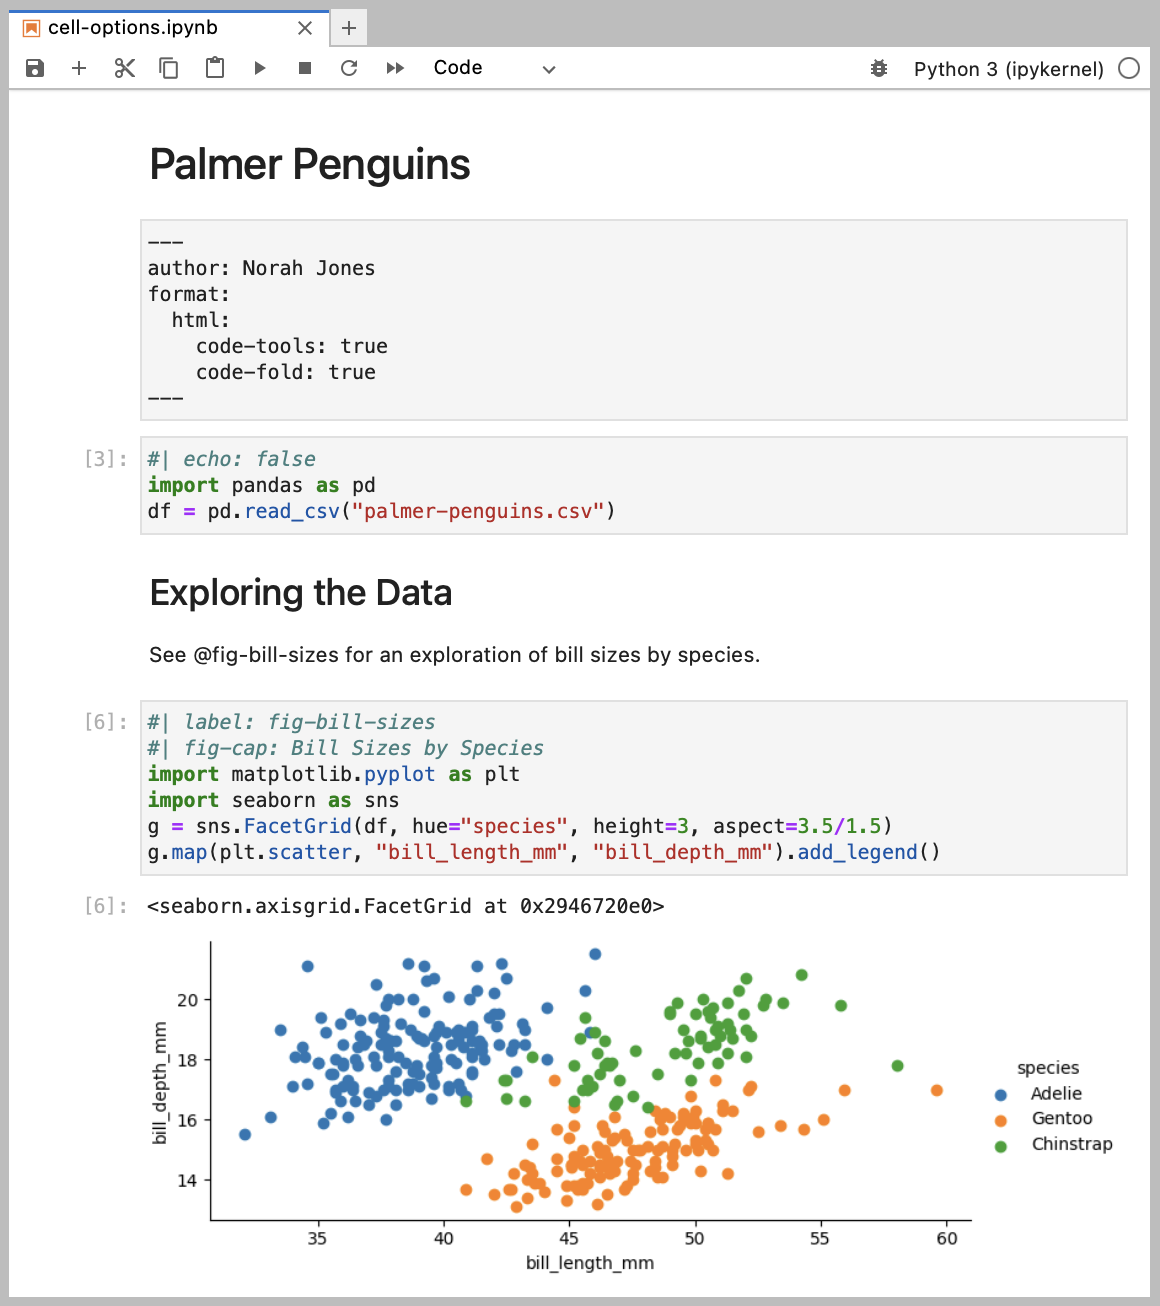
\includegraphics{images/demo-jupyter-plain.png}

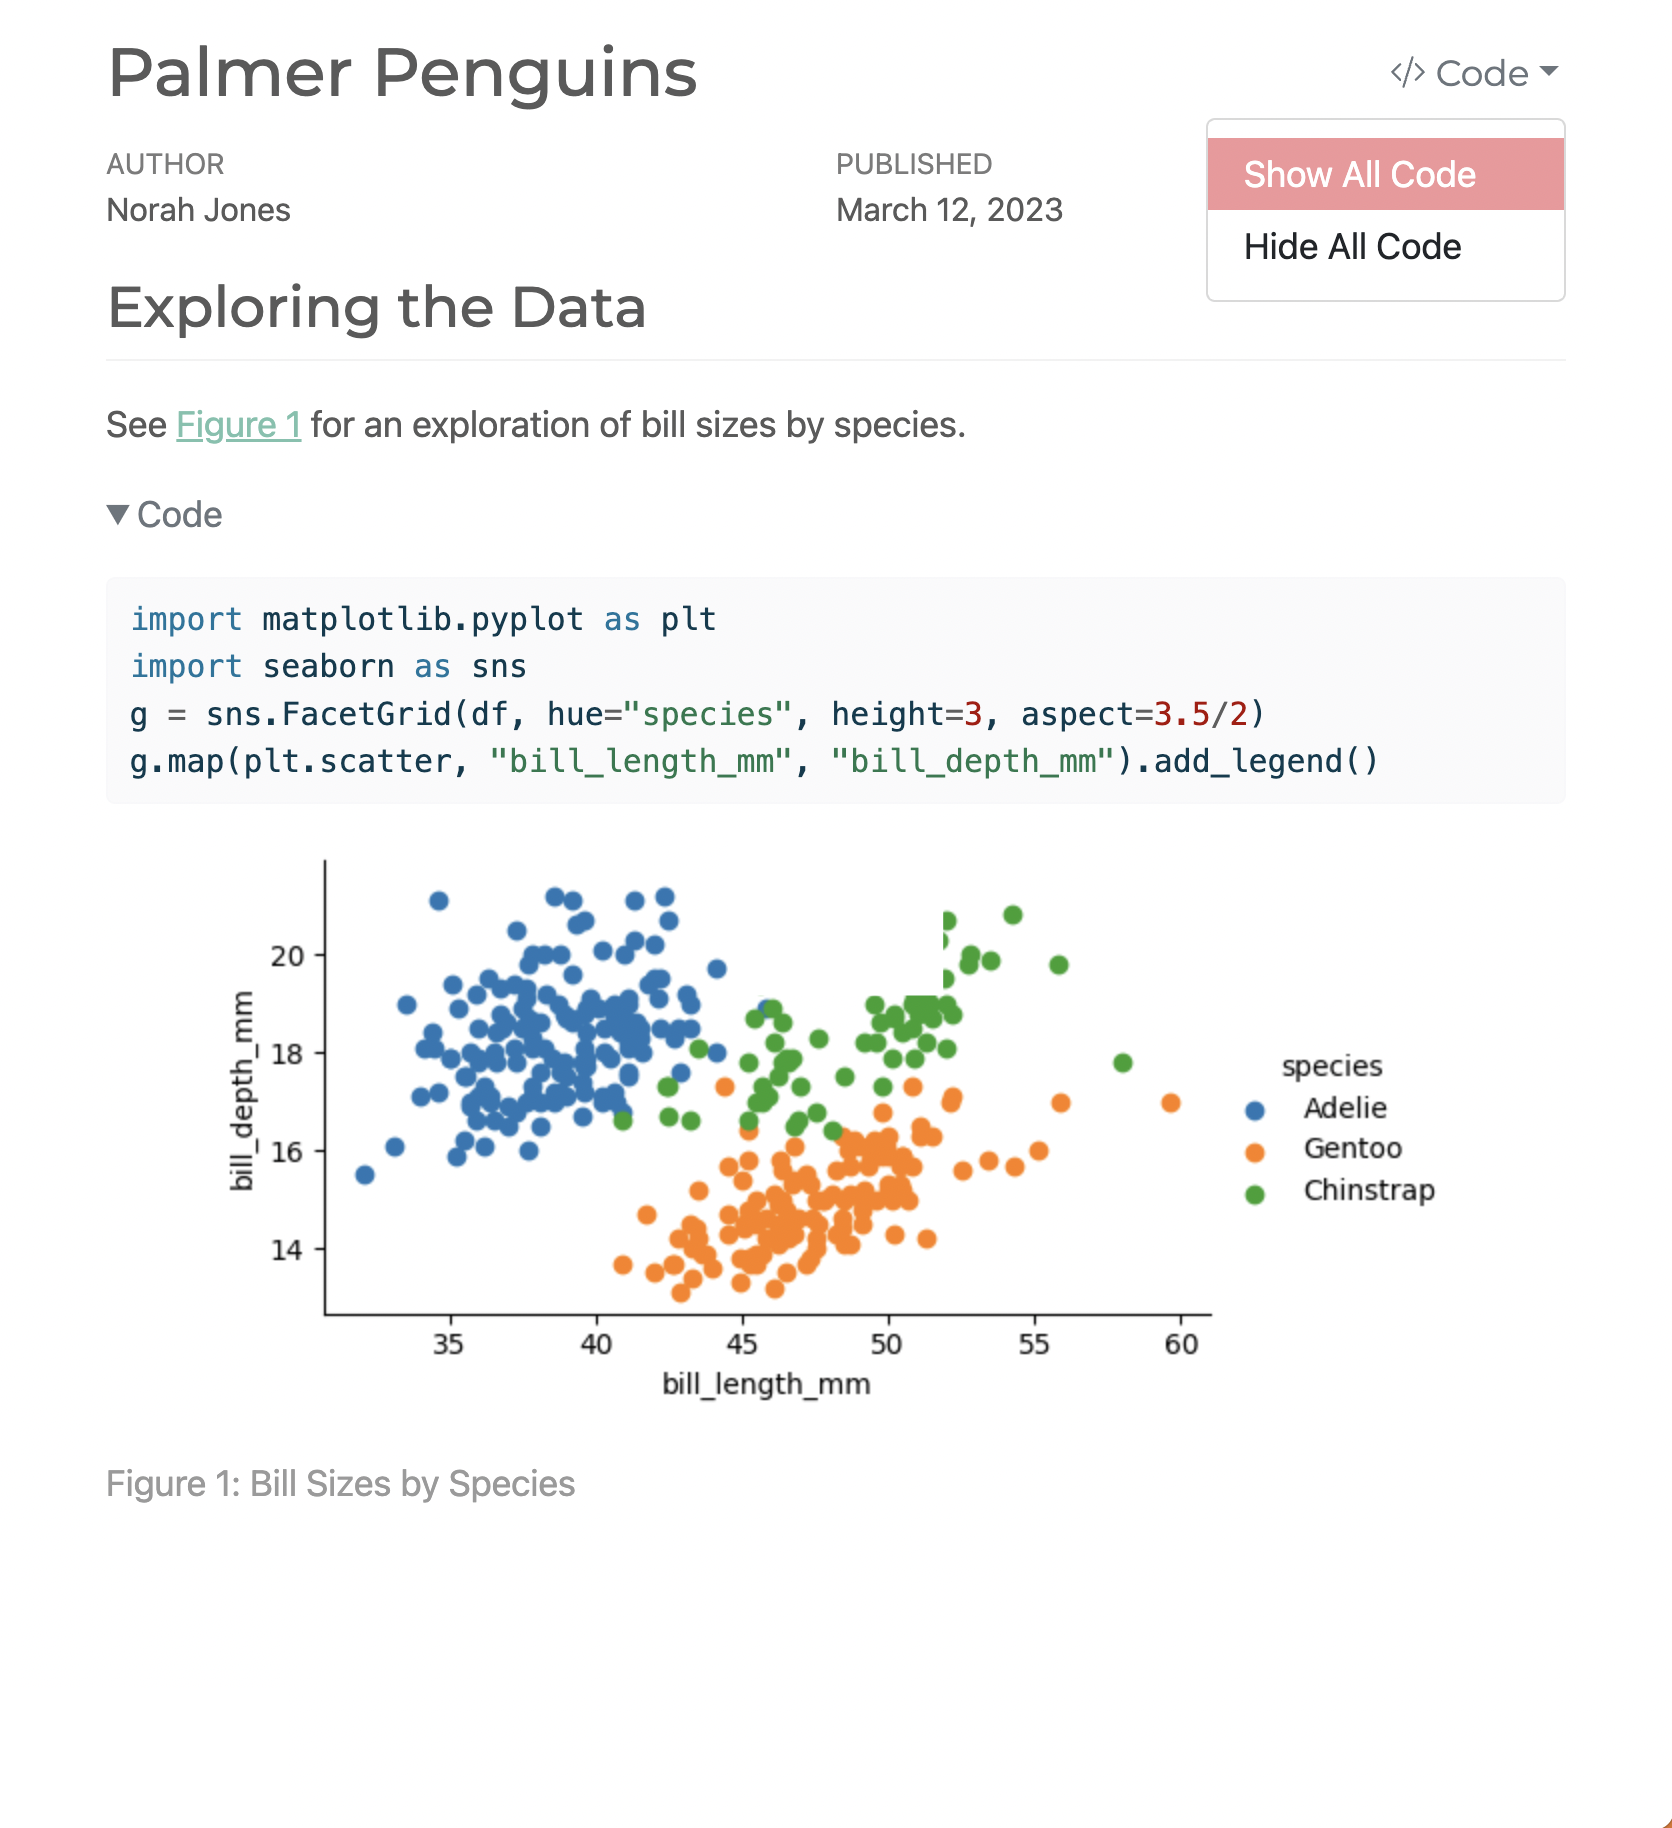
\includegraphics{images/demo-jupyter-output.png}

\leavevmode\vadjust pre{\hypertarget{filosofia}{}}%
La filosofía es una disciplina que busca comprender y cuestionar
aspectos fundamentales de la existencia humana, como la realidad, el
conocimiento, los valores, la moral y la ética. Se ocupa de preguntas
profundas sobre el significado de la vida, la naturaleza del ser, la
verdad y la justicia. La filosofía utiliza el razonamiento lógico y la
reflexión crítica para explorar diferentes perspectivas y argumentos en
busca de respuestas a estos interrogantes.

\begin{Shaded}
\begin{Highlighting}[]
\CommentTok{{-}{-}{-}}
\AnnotationTok{title:}\CommentTok{ "ggplot2 demo"}
\AnnotationTok{author:}\CommentTok{ "Norah Jones"}
\AnnotationTok{date:}\CommentTok{ "5/22/2021"}
\AnnotationTok{format:}\CommentTok{ }
\CommentTok{  html:}
\CommentTok{    fig{-}width: 8}
\CommentTok{    fig{-}height: 4}
\CommentTok{    code{-}fold: true}
\CommentTok{{-}{-}{-}}

\FunctionTok{\#\# Air Quality}

\NormalTok{@fig{-}airquality further explores the impact of temperature on ozone level.}

\InformationTok{\textasciigrave{}\textasciigrave{}\textasciigrave{}\{r\}}
\CommentTok{\#| label: fig{-}airquality}
\CommentTok{\#| fig{-}cap: "Temperature and ozone level."}
\CommentTok{\#| warning: false}

\FunctionTok{library}\NormalTok{(ggplot2)}

\FunctionTok{ggplot}\NormalTok{(airquality, }\FunctionTok{aes}\NormalTok{(Temp, Ozone)) }\SpecialCharTok{+} 
  \FunctionTok{geom\_point}\NormalTok{() }\SpecialCharTok{+} 
  \FunctionTok{geom\_smooth}\NormalTok{(}\AttributeTok{method =} \StringTok{"loess"}
\NormalTok{)}
\InformationTok{\textasciigrave{}\textasciigrave{}\textasciigrave{}}
\end{Highlighting}
\end{Shaded}

\begin{figure}

{\centering 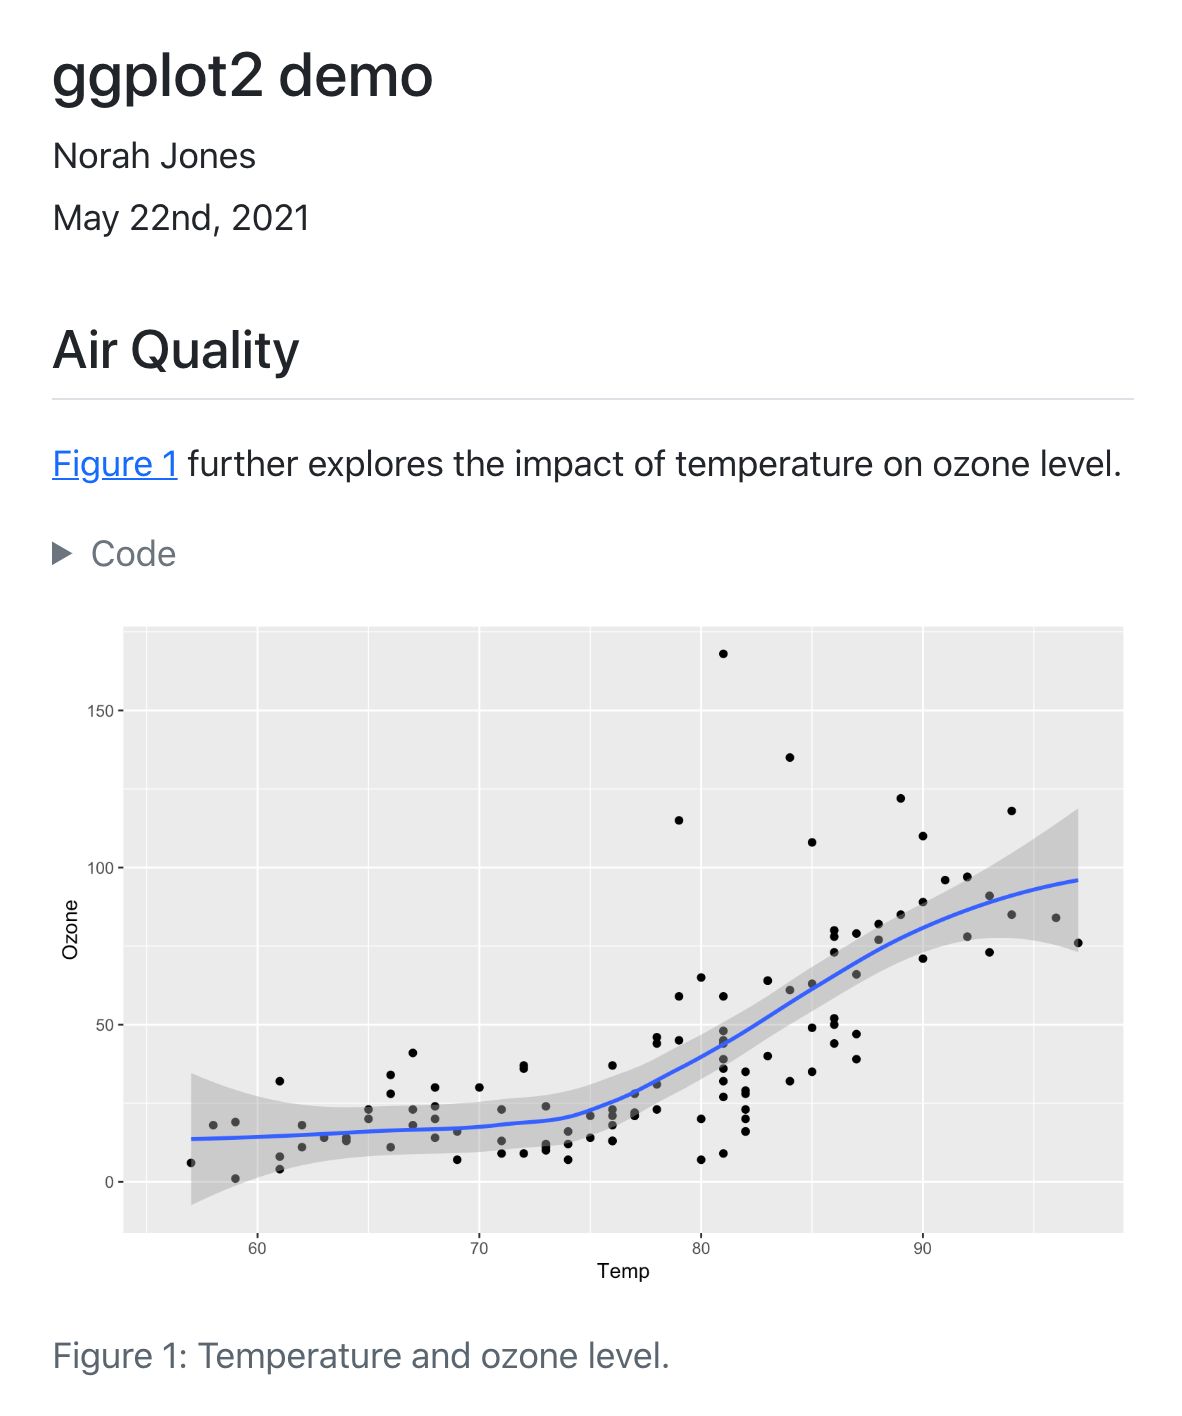
\includegraphics{images/hello-knitr.png}

}

\end{figure}

\leavevmode\vadjust pre{\hypertarget{matematica}{}}%
Las matemáticas son una disciplina que se dedica al estudio de las
propiedades y relaciones de los números, las estructuras abstractas y
los patrones. Se utiliza para describir y analizar fenómenos
cuantitativos en una amplia gama de campos, desde las ciencias naturales
y la ingeniería hasta las ciencias sociales y la economía. Las
matemáticas proporcionan herramientas y métodos para el razonamiento
lógico, la resolución de problemas y el modelado de situaciones
complejas.

\begin{Shaded}
\begin{Highlighting}[]
\CommentTok{{-}{-}{-}}
\AnnotationTok{title:}\CommentTok{ "Plots Demo"}
\AnnotationTok{author:}\CommentTok{ "Norah Jones"}
\AnnotationTok{date:}\CommentTok{ "5/22/2021"}
\AnnotationTok{format:}
\CommentTok{  html:}
\CommentTok{    code{-}fold: true}
\AnnotationTok{jupyter:}\CommentTok{ julia{-}1.8}
\CommentTok{{-}{-}{-}}

\FunctionTok{\#\# Parametric Plots}

\NormalTok{Plot function pair (x(u), y(u)). }
\NormalTok{See @fig{-}parametric for an example.}

\InformationTok{\textasciigrave{}\textasciigrave{}\textasciigrave{}\{julia\}}
\CommentTok{\#| label: fig{-}parametric}
\CommentTok{\#| fig{-}cap: "Parametric Plots"}

\NormalTok{using Plots}

\NormalTok{plot(}\FunctionTok{sin}\NormalTok{, }
\NormalTok{     x{-}\textgreater{}}\FunctionTok{sin}\NormalTok{(}\DecValTok{2}\NormalTok{x), }
     \DecValTok{0}\NormalTok{, }
     \DecValTok{2}\NormalTok{π, }
\NormalTok{     leg=false, }
\NormalTok{     fill=(}\DecValTok{0}\NormalTok{,:lavender))}
\InformationTok{\textasciigrave{}\textasciigrave{}\textasciigrave{}}
\end{Highlighting}
\end{Shaded}

\begin{figure}

{\centering 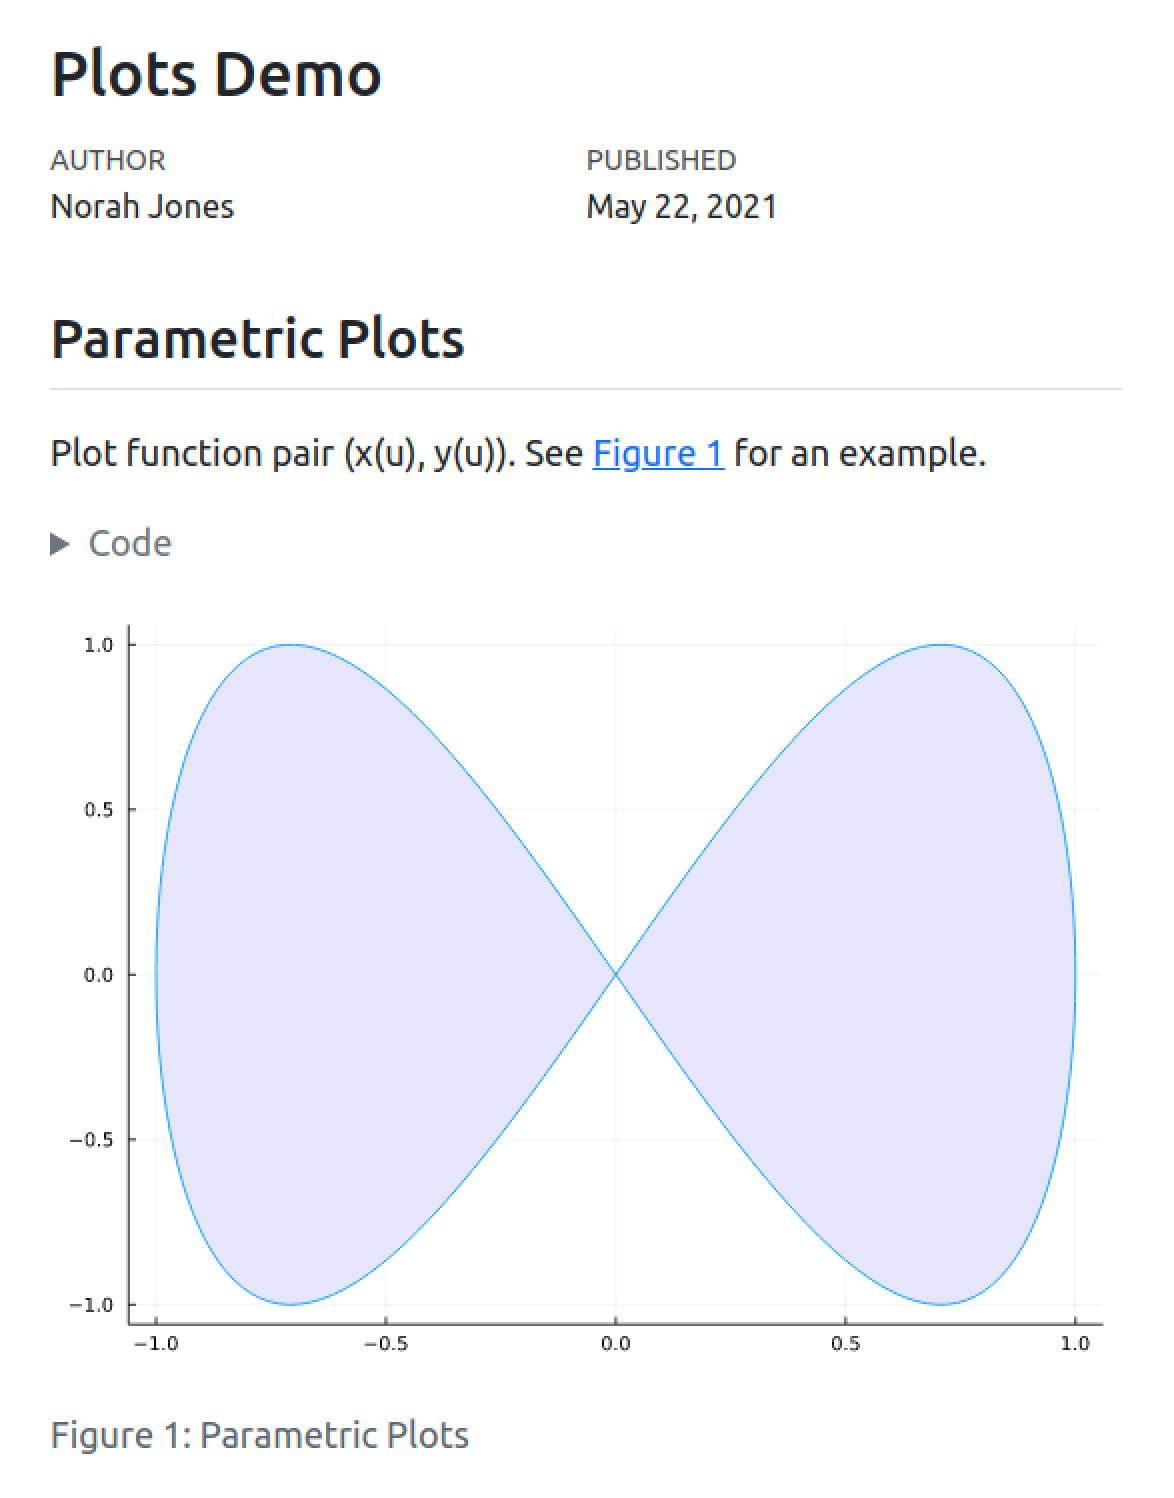
\includegraphics{images/hello-julia.png}

}

\end{figure}

\leavevmode\vadjust pre{\hypertarget{informatica}{}}%
La informática es una disciplina que se ocupa del estudio y desarrollo
de sistemas de información y computación. Comprende el diseño, la
programación, la gestión y el uso de sistemas y software para procesar,
almacenar y transmitir información de manera eficiente. La informática
abarca áreas como la programación, las bases de datos, la inteligencia
artificial, la seguridad informática y el desarrollo de aplicaciones y
sistemas. Su objetivo principal es aprovechar la tecnología de la
información para resolver problemas y mejorar la eficiencia en diversos
ámbitos de la sociedad.

\begin{Shaded}
\begin{Highlighting}[]
\CommentTok{{-}{-}{-}}
\AnnotationTok{title:}\CommentTok{ "observable plot"}
\AnnotationTok{author:}\CommentTok{ "Norah Jones"}
\AnnotationTok{format:}\CommentTok{ }
\CommentTok{  html: }
\CommentTok{    code{-}fold: true}
\CommentTok{{-}{-}{-}}

\FunctionTok{\#\# Seattle Precipitation by Day (2012 to 2016)}

\InformationTok{\textasciigrave{}\textasciigrave{}\textasciigrave{}\{ojs\}}
\NormalTok{data }\OperatorTok{=} \FunctionTok{FileAttachment}\NormalTok{(}\StringTok{"seattle{-}weather.csv"}\NormalTok{)}
  \OperatorTok{.}\FunctionTok{csv}\NormalTok{(\{}\DataTypeTok{typed}\OperatorTok{:} \KeywordTok{true}\NormalTok{\})}
  
\NormalTok{Plot}\OperatorTok{.}\FunctionTok{plot}\NormalTok{(\{}
  \DataTypeTok{width}\OperatorTok{:} \DecValTok{800}\OperatorTok{,} \DataTypeTok{height}\OperatorTok{:} \DecValTok{500}\OperatorTok{,} \DataTypeTok{padding}\OperatorTok{:} \DecValTok{0}\OperatorTok{,}
  \DataTypeTok{color}\OperatorTok{:}\NormalTok{ \{ }\DataTypeTok{scheme}\OperatorTok{:} \StringTok{"blues"}\OperatorTok{,} \DataTypeTok{type}\OperatorTok{:} \StringTok{"sqrt"}\NormalTok{\}}\OperatorTok{,}
  \DataTypeTok{y}\OperatorTok{:}\NormalTok{ \{ }\DataTypeTok{tickFormat}\OperatorTok{:}\NormalTok{ i }\KeywordTok{=\textgreater{}} \StringTok{"JFMAMJJASOND"}\NormalTok{[i] \}}\OperatorTok{,}
  \DataTypeTok{marks}\OperatorTok{:}\NormalTok{ [}
\NormalTok{    Plot}\OperatorTok{.}\FunctionTok{cell}\NormalTok{(data}\OperatorTok{,}\NormalTok{ Plot}\OperatorTok{.}\FunctionTok{group}\NormalTok{(\{}\DataTypeTok{fill}\OperatorTok{:} \StringTok{"mean"}\NormalTok{\}}\OperatorTok{,}\NormalTok{ \{}
      \DataTypeTok{x}\OperatorTok{:}\NormalTok{ d }\KeywordTok{=\textgreater{}}\NormalTok{ d}\OperatorTok{.}\AttributeTok{date}\OperatorTok{.}\FunctionTok{getUTCDate}\NormalTok{()}\OperatorTok{,}
      \DataTypeTok{y}\OperatorTok{:}\NormalTok{ d }\KeywordTok{=\textgreater{}}\NormalTok{ d}\OperatorTok{.}\AttributeTok{date}\OperatorTok{.}\FunctionTok{getUTCMonth}\NormalTok{()}\OperatorTok{,}
      \DataTypeTok{fill}\OperatorTok{:} \StringTok{"precipitation"}\OperatorTok{,} 
      \DataTypeTok{inset}\OperatorTok{:} \FloatTok{0.5}
\NormalTok{    \}))}
\NormalTok{  ]}
\NormalTok{\})}
\VerbatimStringTok{\textasciigrave{}\textasciigrave{}\textasciigrave{}}
\end{Highlighting}
\end{Shaded}

\begin{figure}

{\centering 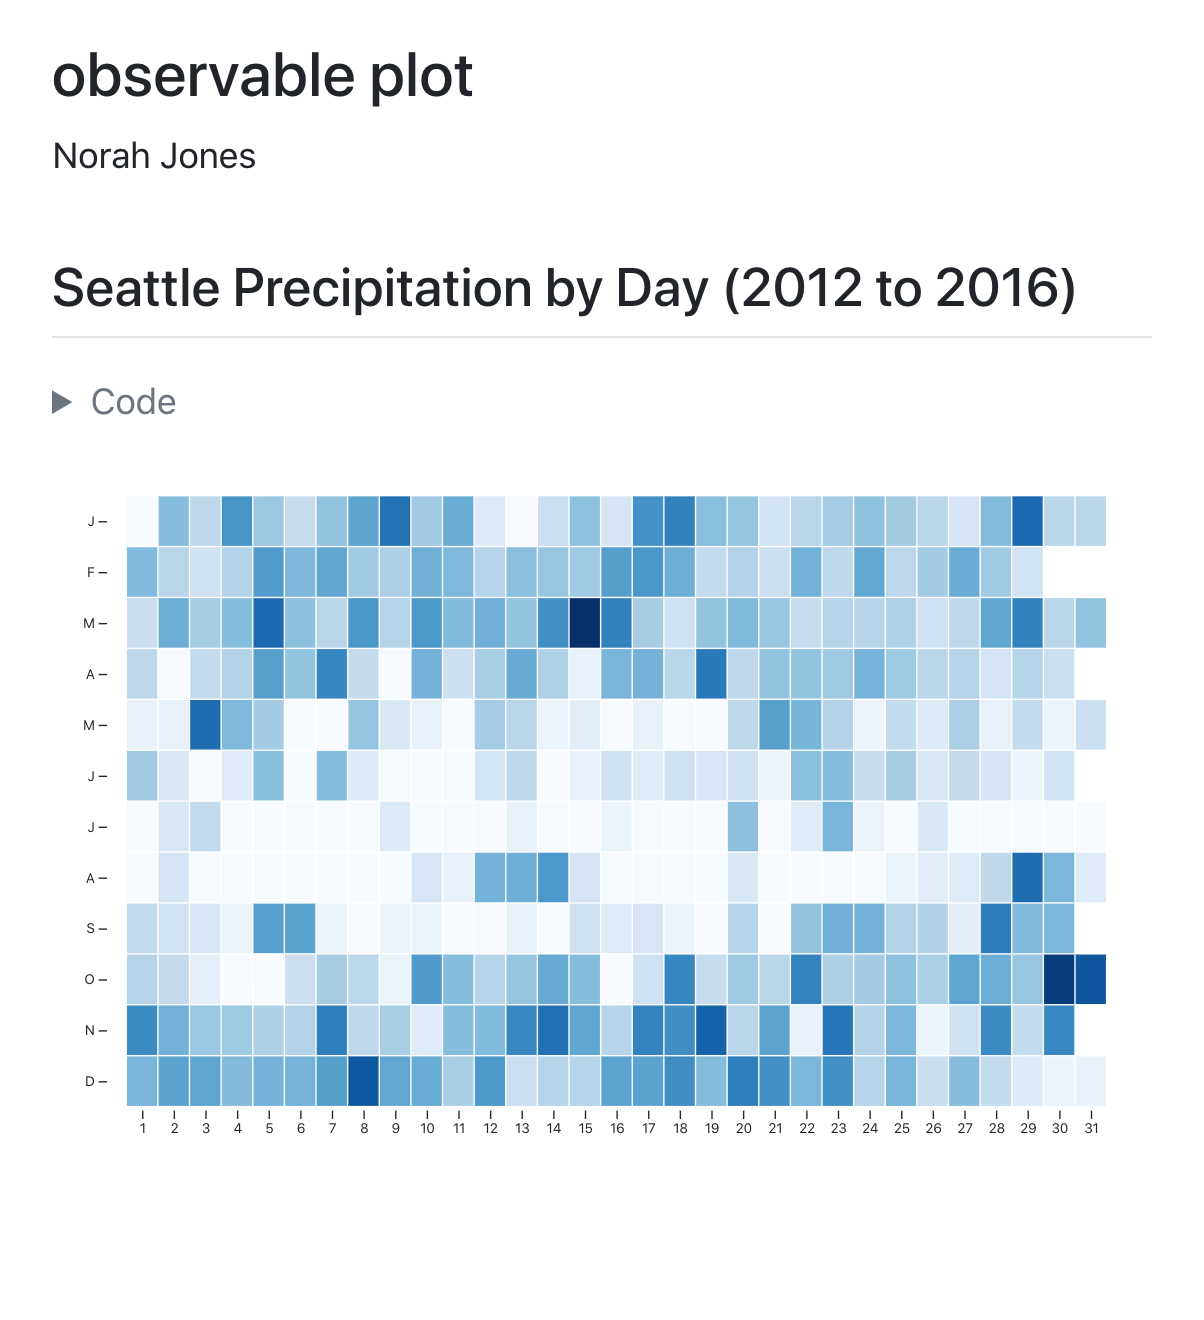
\includegraphics{images/hello-observable.png}

}

\end{figure}

\href{docs/get-started/index.html}{Sobre mi}


\printbibliography


\end{document}
